\chapter{Utilizzo del Protocollo DATEX II}
\label{app:a}
In questo appendice sono mostrati  i diagrammi delle classi relativi all'utilizzo del Protocollo DATEX II all'interno del sistema definito nel \autoref{chap:tre}.\\
I diagrammi delle classi di seguito mostrati sono stati ricavati da quelli progettati per lo standard DATEX. (\url{http://d2docs.ndwcloud.nu/_static/umlmodel/v3.0/index.htm})\\
Si presti inoltre attenzione al fatto che i diagrammi delle classi mostrati in questo appendice non coprono il progetto nella sua interezza ma si intendono riferite alla sola implementazione dello standard DATEX II all'interno del progetto.
Infine, i diagrammi delle classi di seguito esposti non comprendono lo standard DATEX II nella sua interezza, ma riguardano le sole componenti che si è ritenuto opportuno integrare nel progetto.\\
\subsubsection{General Structure}
\begin{figure}
	\begin{center}
		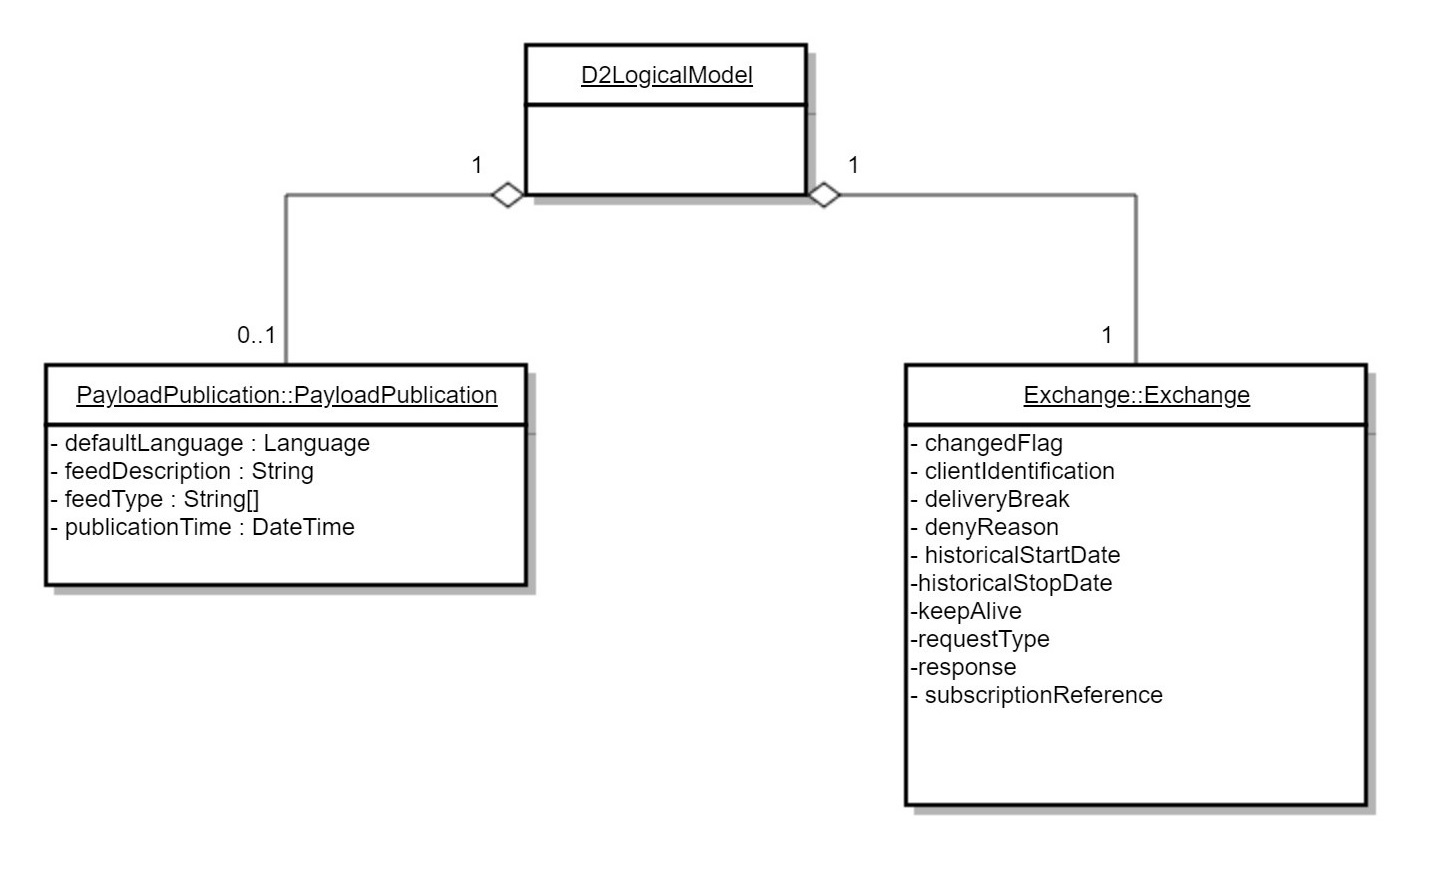
\includegraphics[width=0.6\columnwidth]{images/uml_1}
	\end{center}
	\caption{Distinzione effettuata dallo Standard DATEX II tra metodo di comunicazione (\textit{Exchange}) e formato del Payload (\textit{PayloadPublication})}
	\label{fig:app_uml_1}
\end{figure}
\begin{figure}
	\begin{center}
		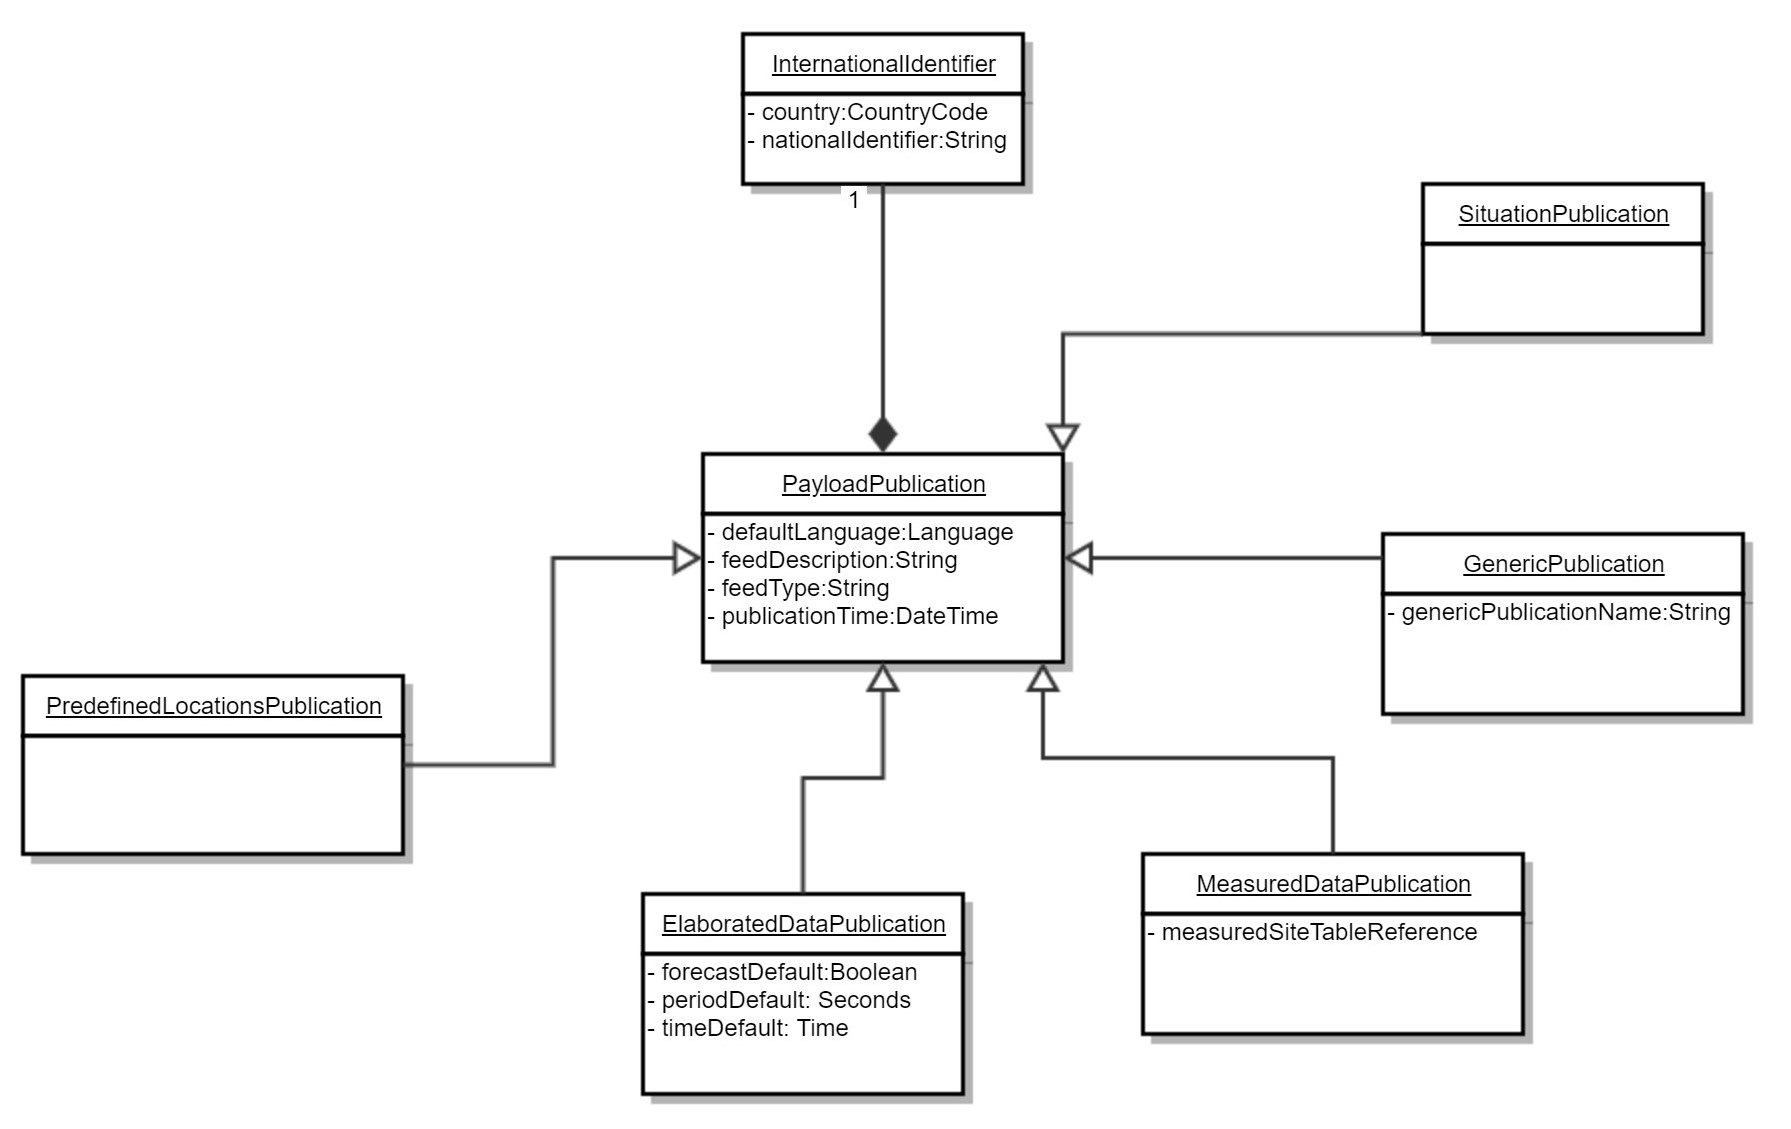
\includegraphics[width=0.9\columnwidth]{images/datexii_publication_implementation}
	\end{center}
	\caption{Implementazione della Publication}
	\label{fig:app_datexii_publication_implementation}
\end{figure}
\begin{figure}
	\begin{center}
		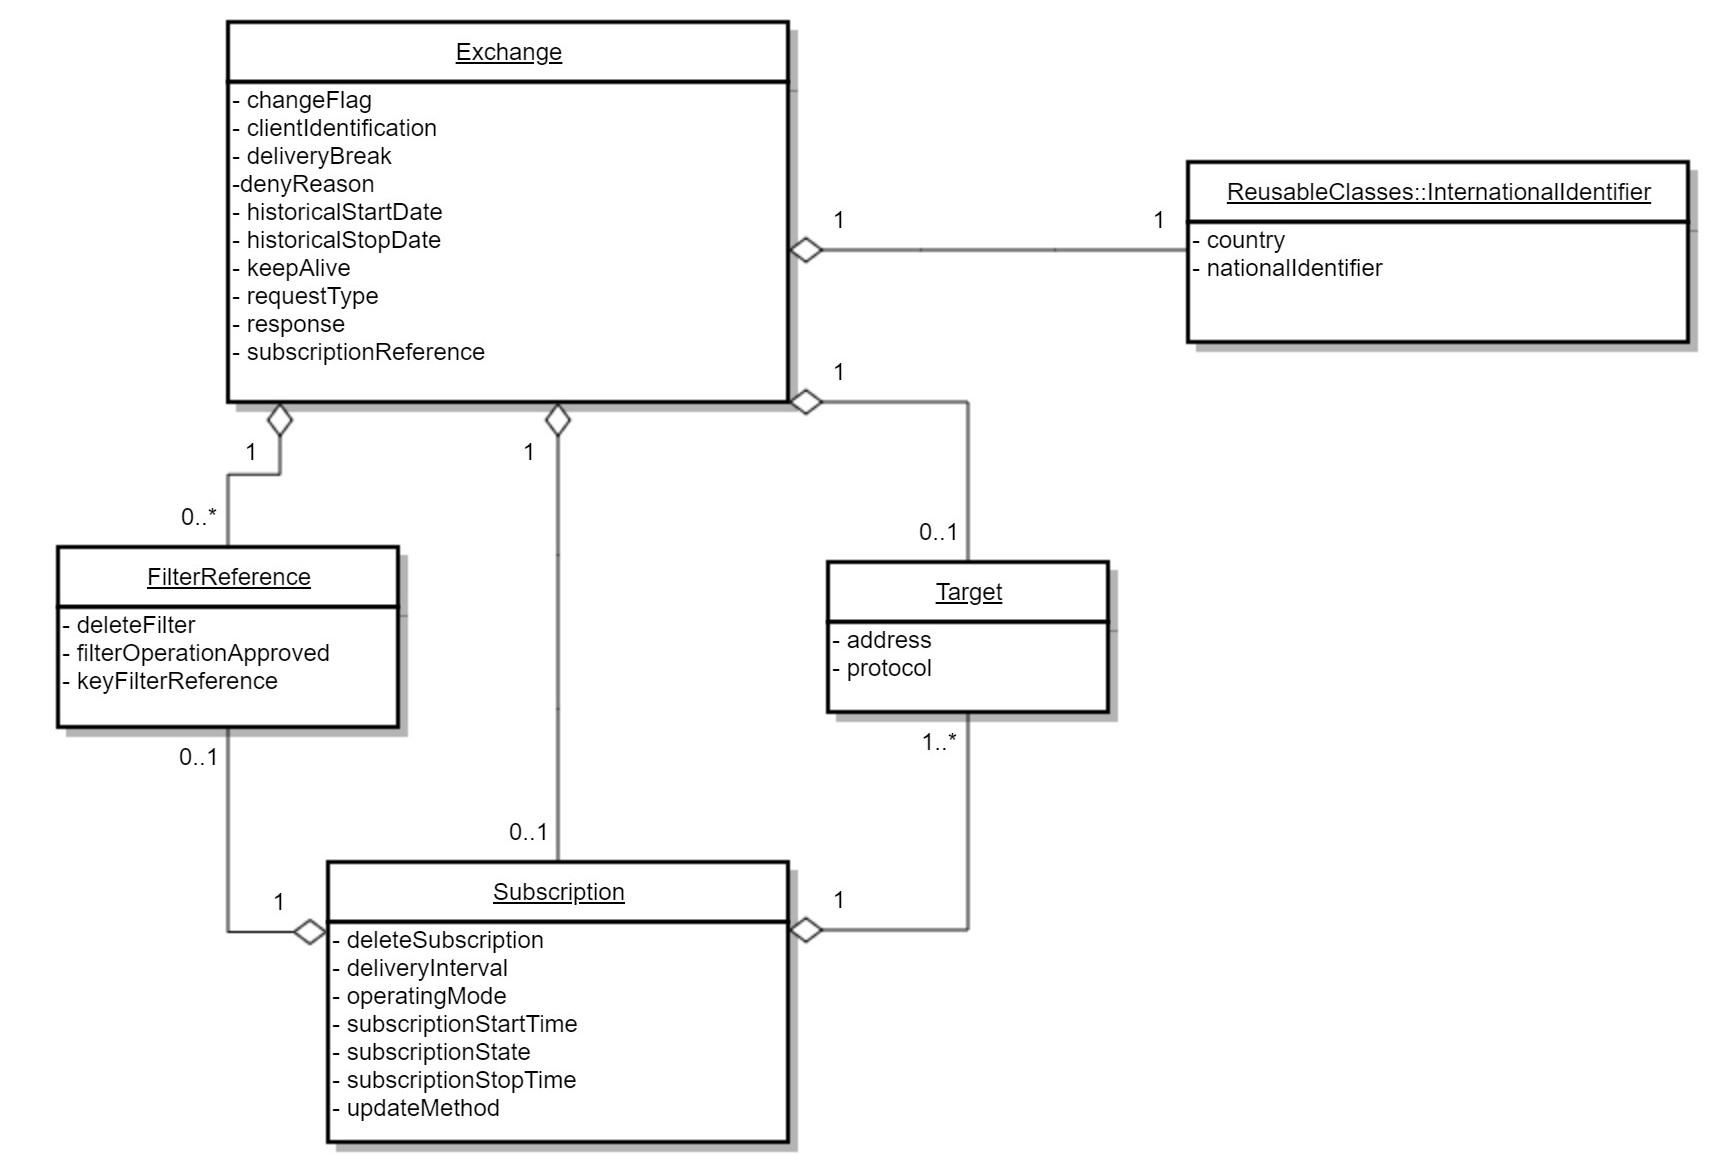
\includegraphics[width=0.8\columnwidth]{images/uml_2}
	\end{center}
	\caption{Implementazione del' Exchange}
	\label{fig:app_uml_2}
\end{figure}
\subsubsection{Location}
\begin{figure}
	\begin{center}
		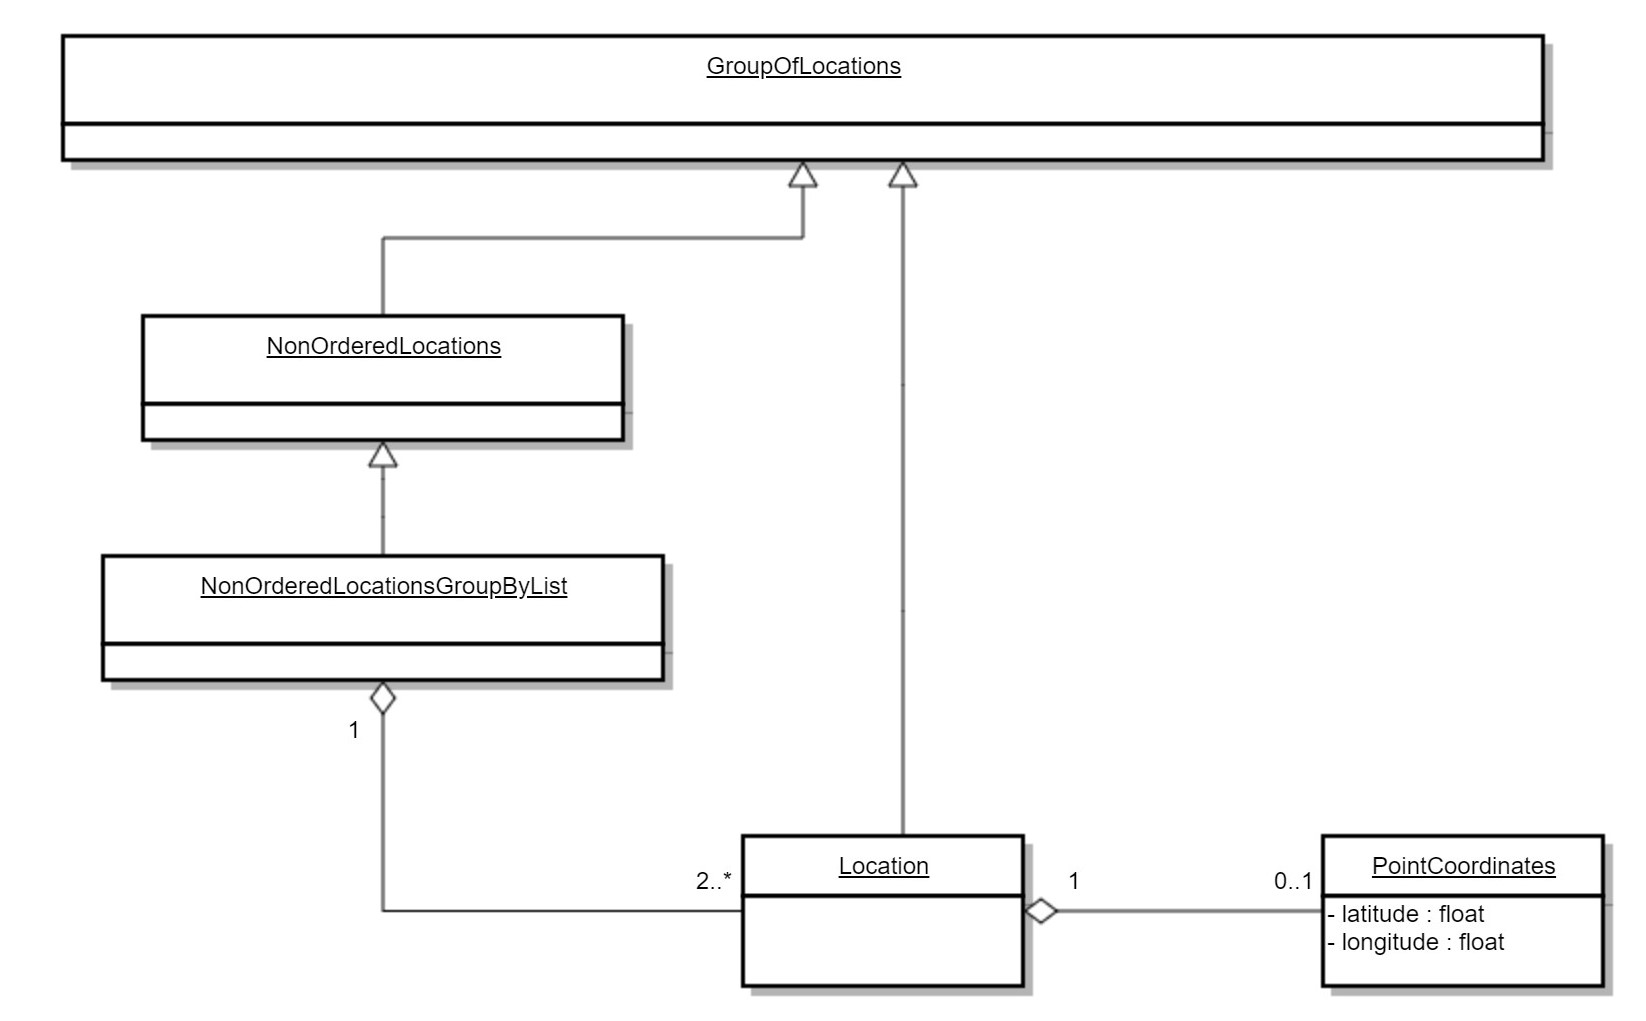
\includegraphics[width=1\columnwidth]{images/uml_3_3}
	\end{center}
	\caption{Location reference}
	\label{fig:app_uml_3_3}
\end{figure}
\subsubsection{Elaborated Data Publication}
\begin{figure}
	\begin{center}
		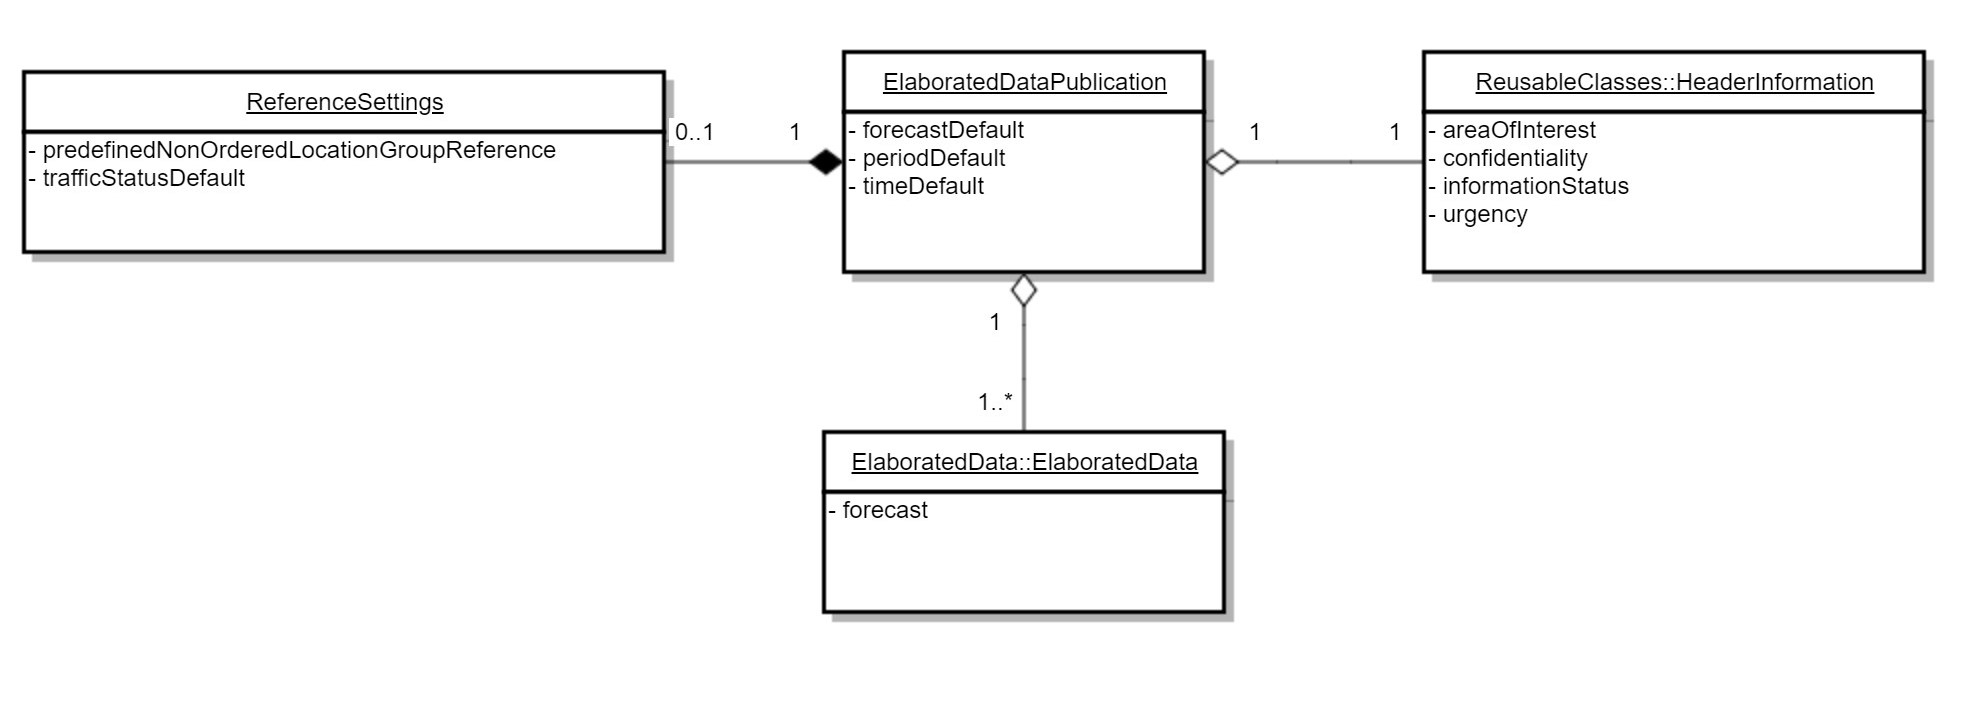
\includegraphics[width=1\columnwidth]{images/uml_3_6}
	\end{center}
	\caption{Elaborated Data Publication structure}
	\label{fig:app_uml_3_6}
\end{figure}
\begin{figure}
	\begin{center}
		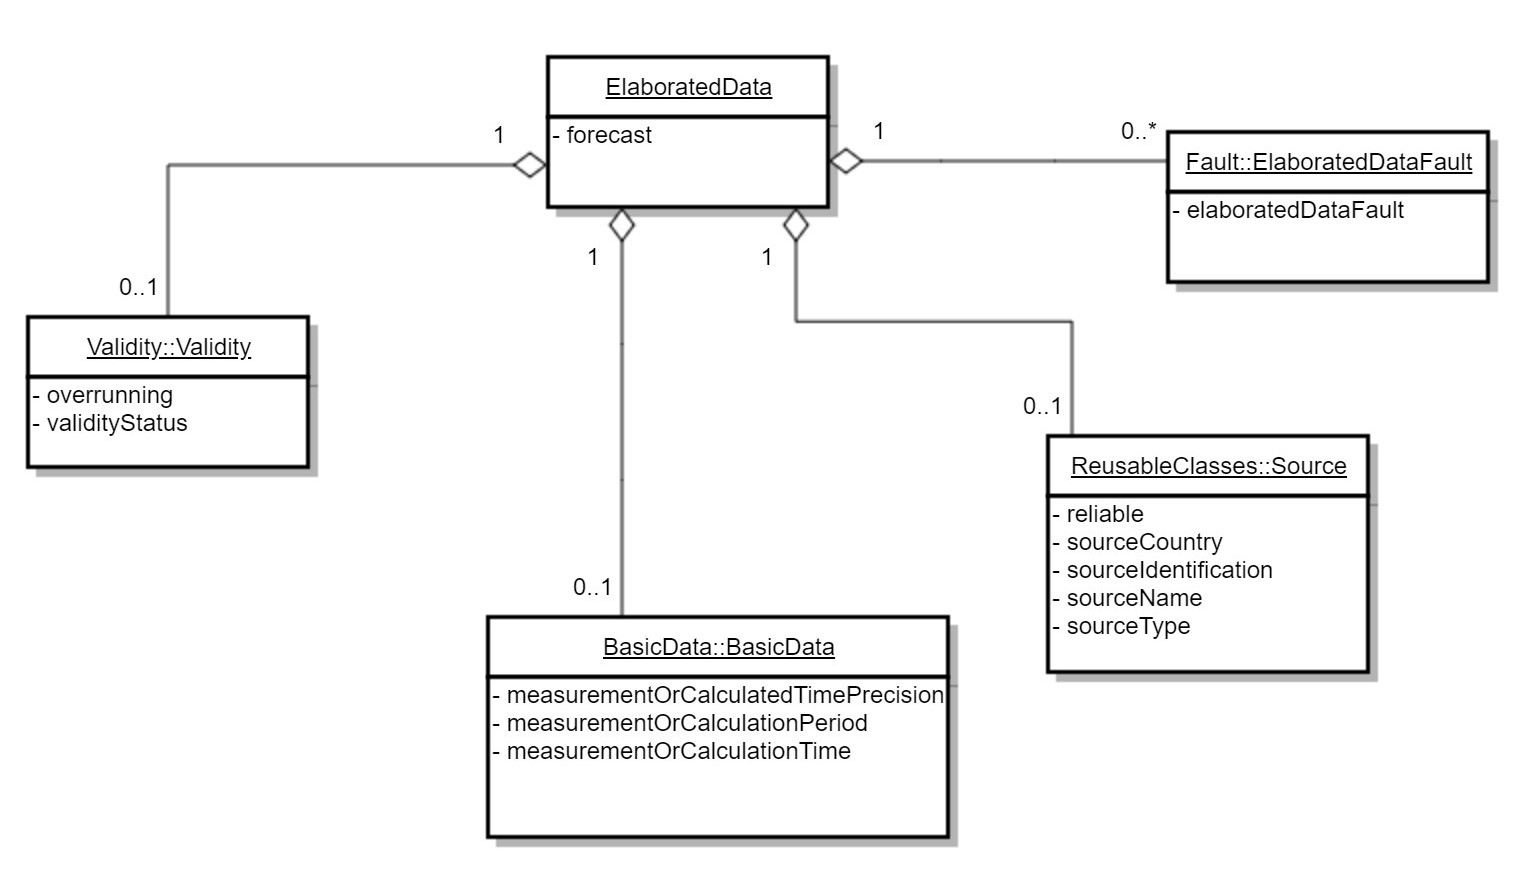
\includegraphics[width=0.7\columnwidth]{images/uml_4_30}
	\end{center}
	\caption{Elaborated Data Implementation}
	\label{fig:app_uml_4_30}
\end{figure}
\subsubsection{Measured Data Publication}
\begin{figure}
	\begin{center}
		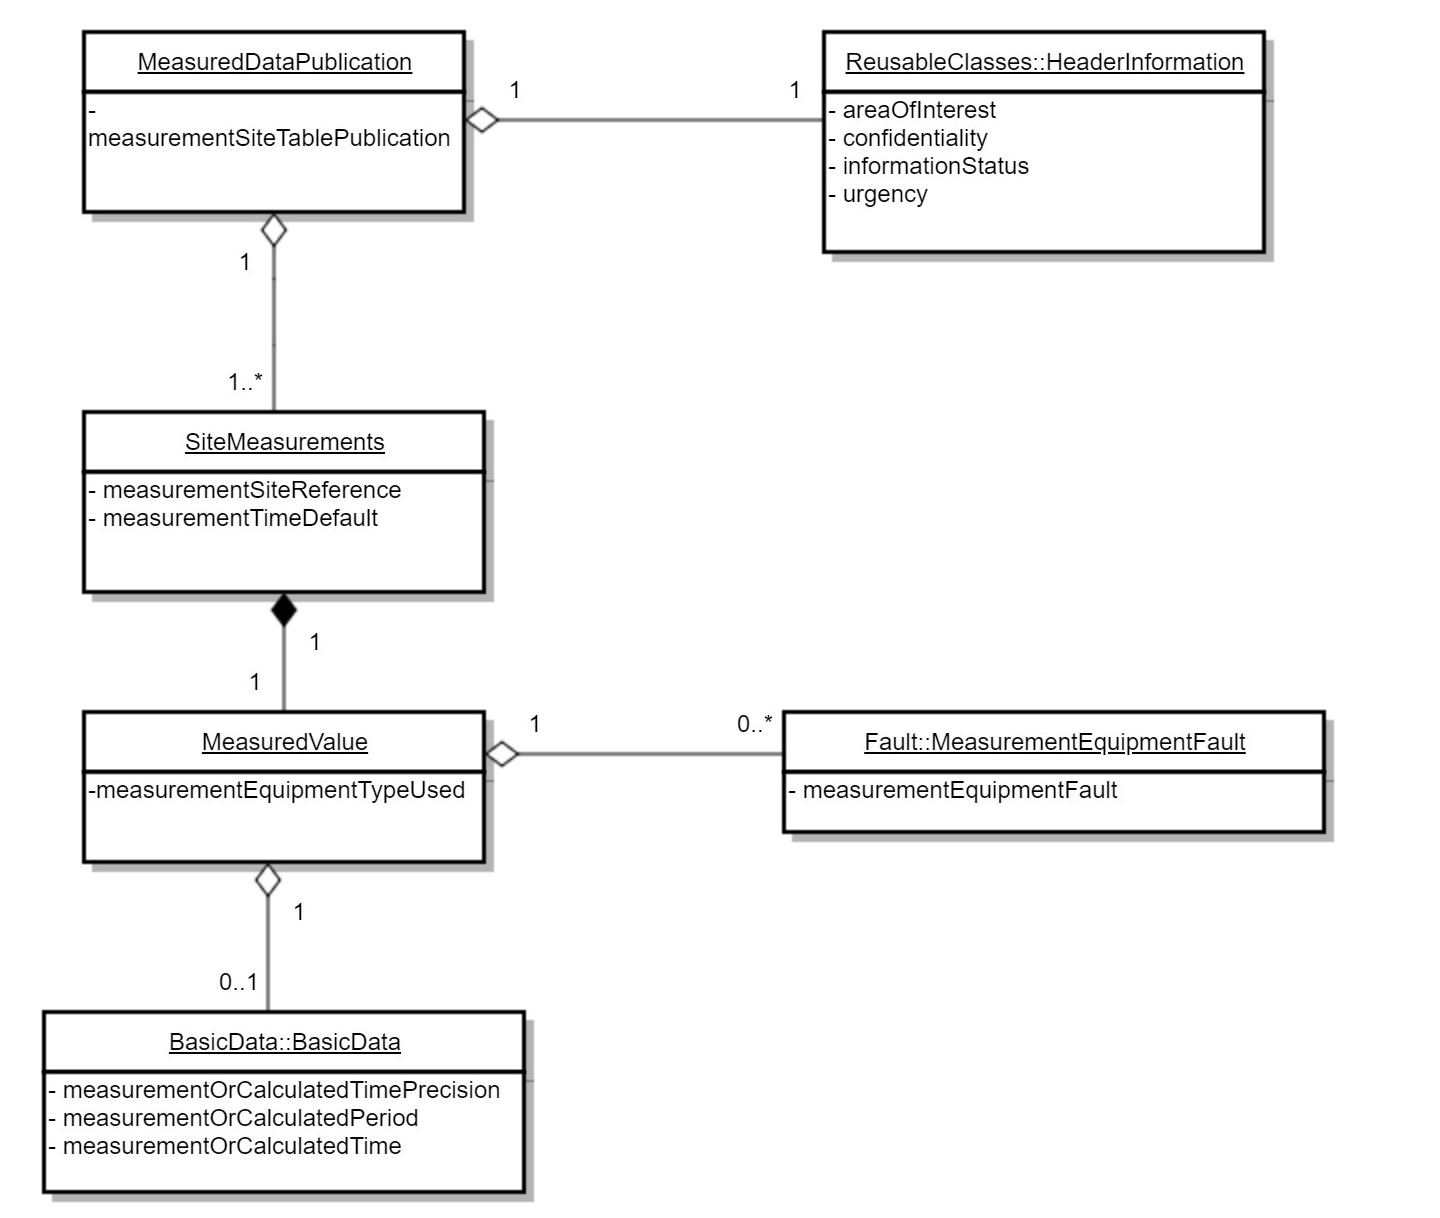
\includegraphics[width=0.8\columnwidth]{images/uml_3_8}
	\end{center}
	\caption{Measured Data Structure}
	\label{fig:app_uml_3_8}
\end{figure}
\begin{figure}
	\begin{center}
		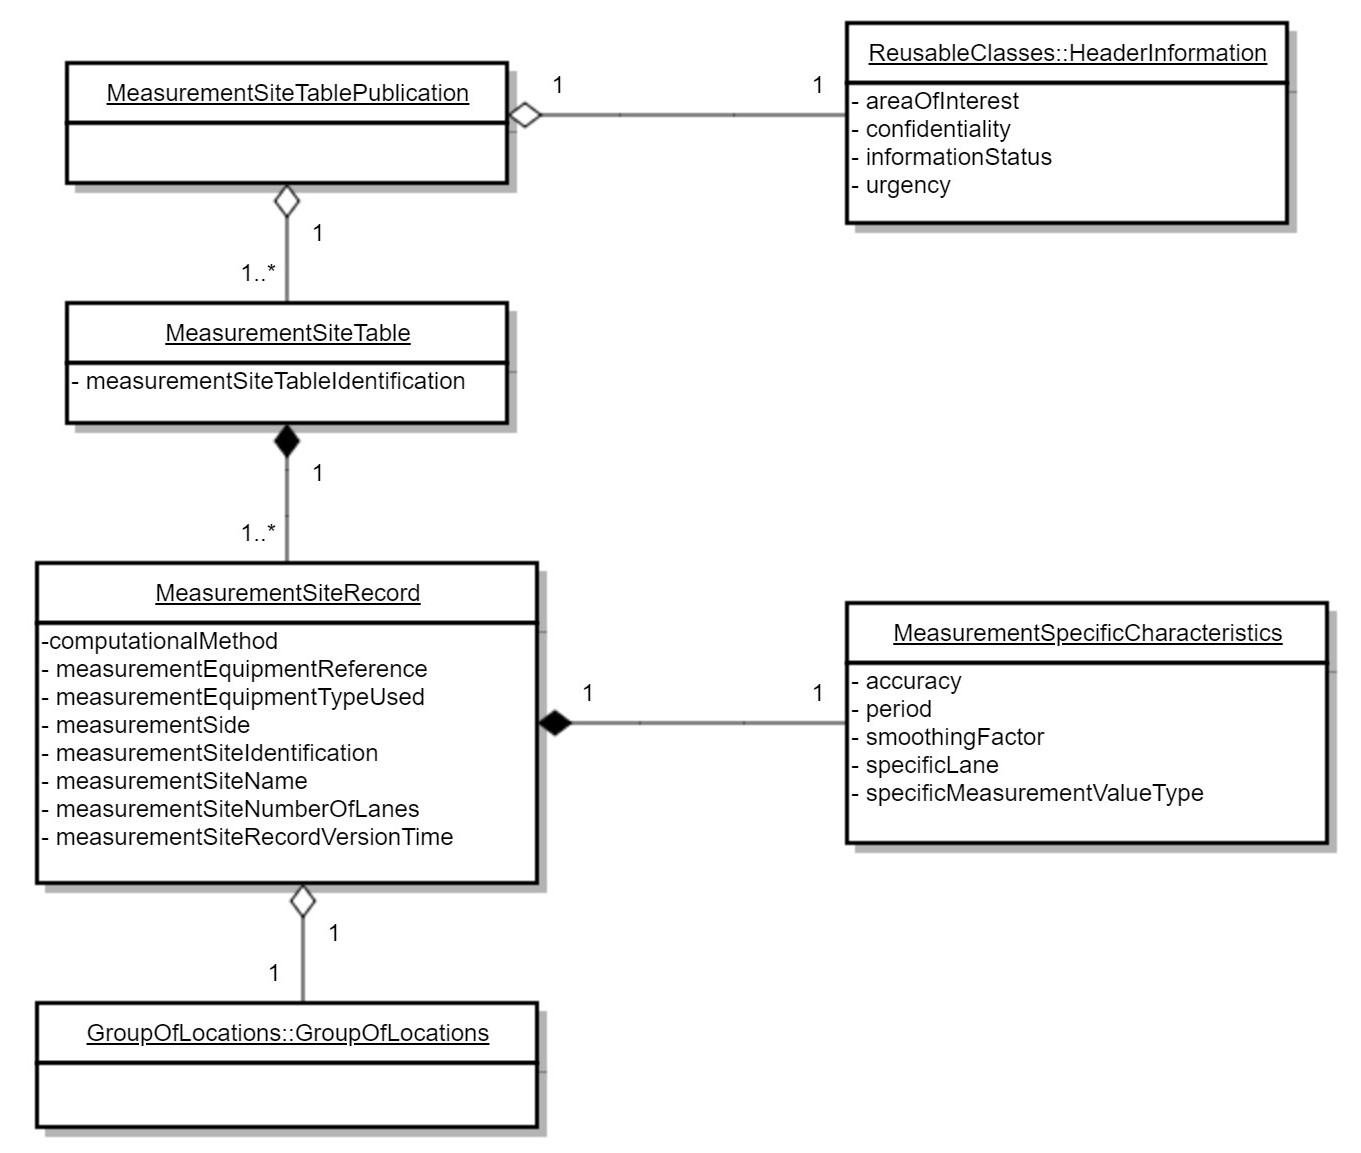
\includegraphics[width=0.75\columnwidth]{images/uml_3_9}
	\end{center}
	\caption{Measurement Site Record Structure}
	\label{fig:app_uml_3_9}
\end{figure}
\begin{figure}
	\begin{center}
		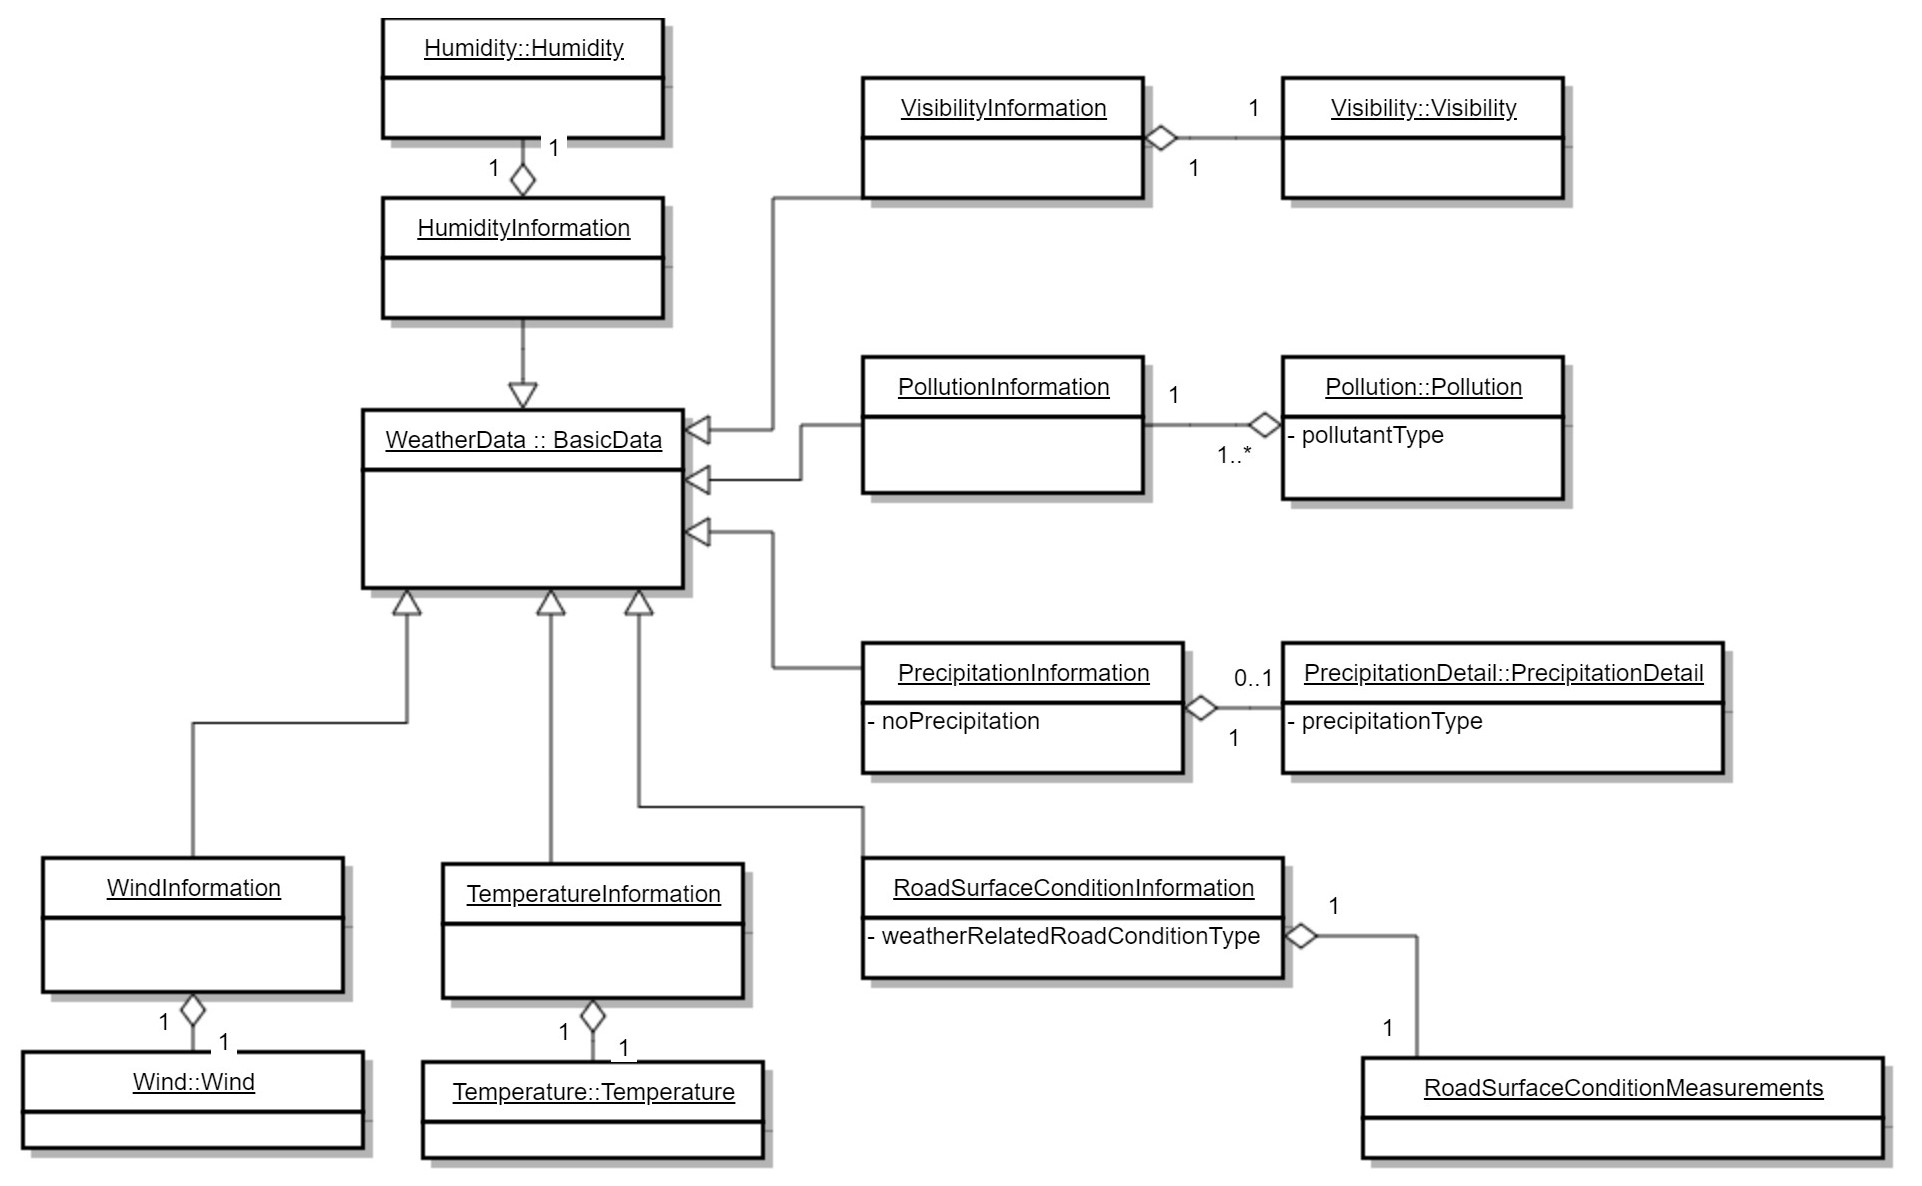
\includegraphics[width=0.8\columnwidth]{images/uml_4_28}
	\end{center}
	\caption{Basic Data Default Implementation}
	\label{fig:app_uml_4_28}
\end{figure}
\begin{figure}
	\begin{center}
		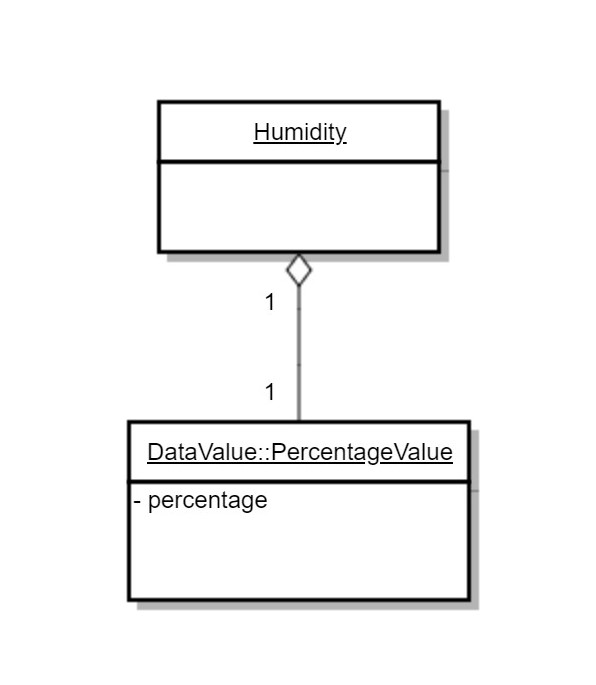
\includegraphics[width=0.5\columnwidth]{images/uml_5_14}
	\end{center}
	\caption{Humidity Implementation}
	\label{fig:app_uml_5_14}
\end{figure}
\begin{figure}
	\begin{center}
		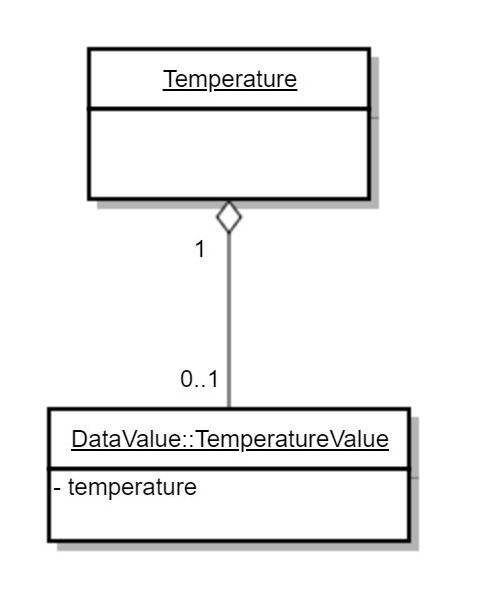
\includegraphics[width=0.45\columnwidth]{images/uml_5_18}
	\end{center}
	\caption{Temperature Implementation}
	\label{fig:app_uml_5_18}
\end{figure}
\begin{figure}
	\begin{center}
		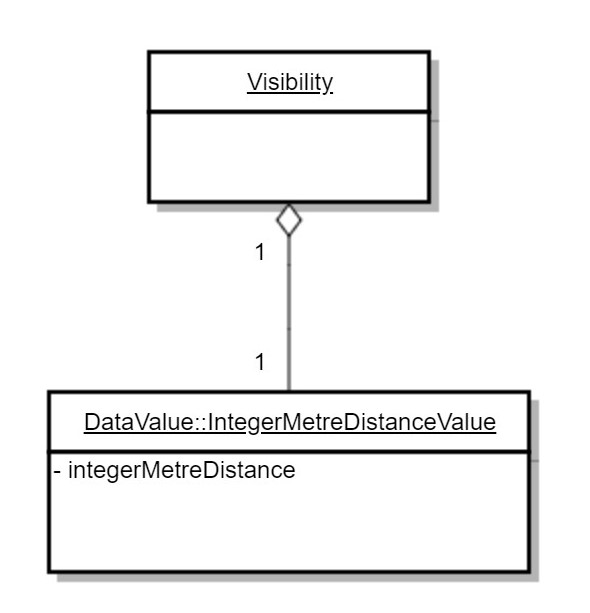
\includegraphics[width=0.65\columnwidth]{images/uml_5_19}
	\end{center}
	\caption{Visibility Implementation}
	\label{fig:app_uml_5_19}
\end{figure}
\begin{figure}
	\begin{center}
		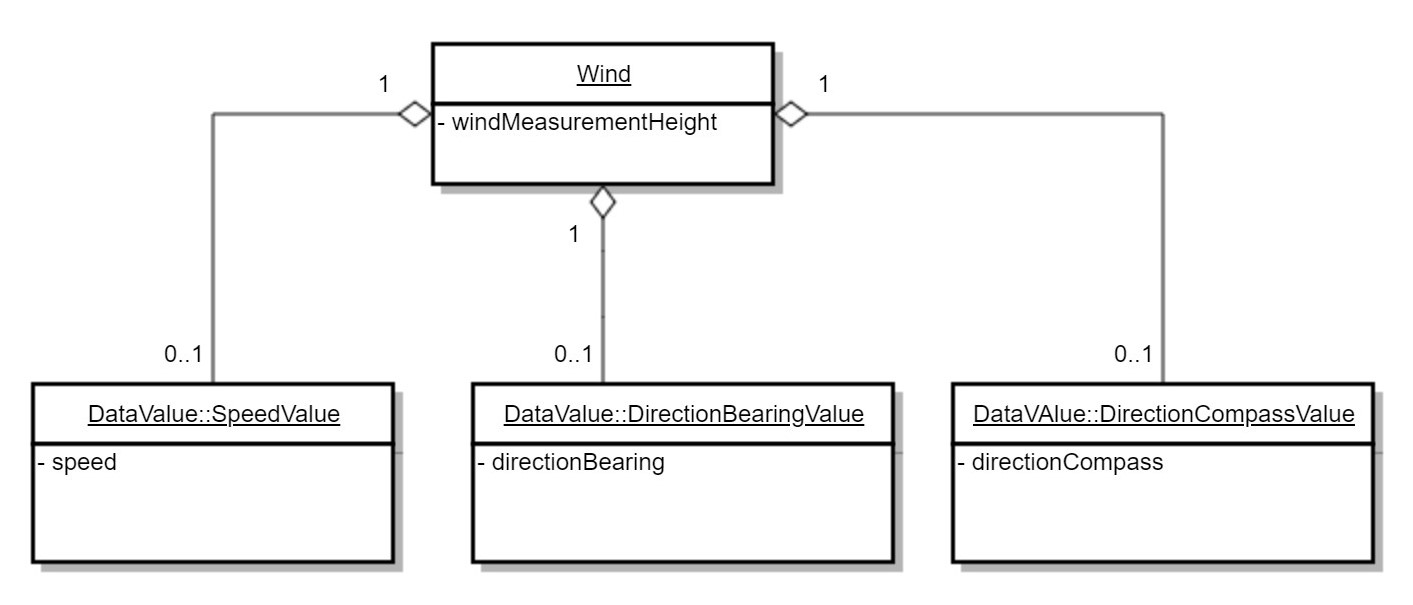
\includegraphics[width=1.1\columnwidth]{images/uml_5_20}
	\end{center}
	\caption{Wind Implementation}
	\label{fig:app_uml_5_20}
\end{figure}
\subsubsection{Situation Publication}
\begin{figure}
	\begin{center}
		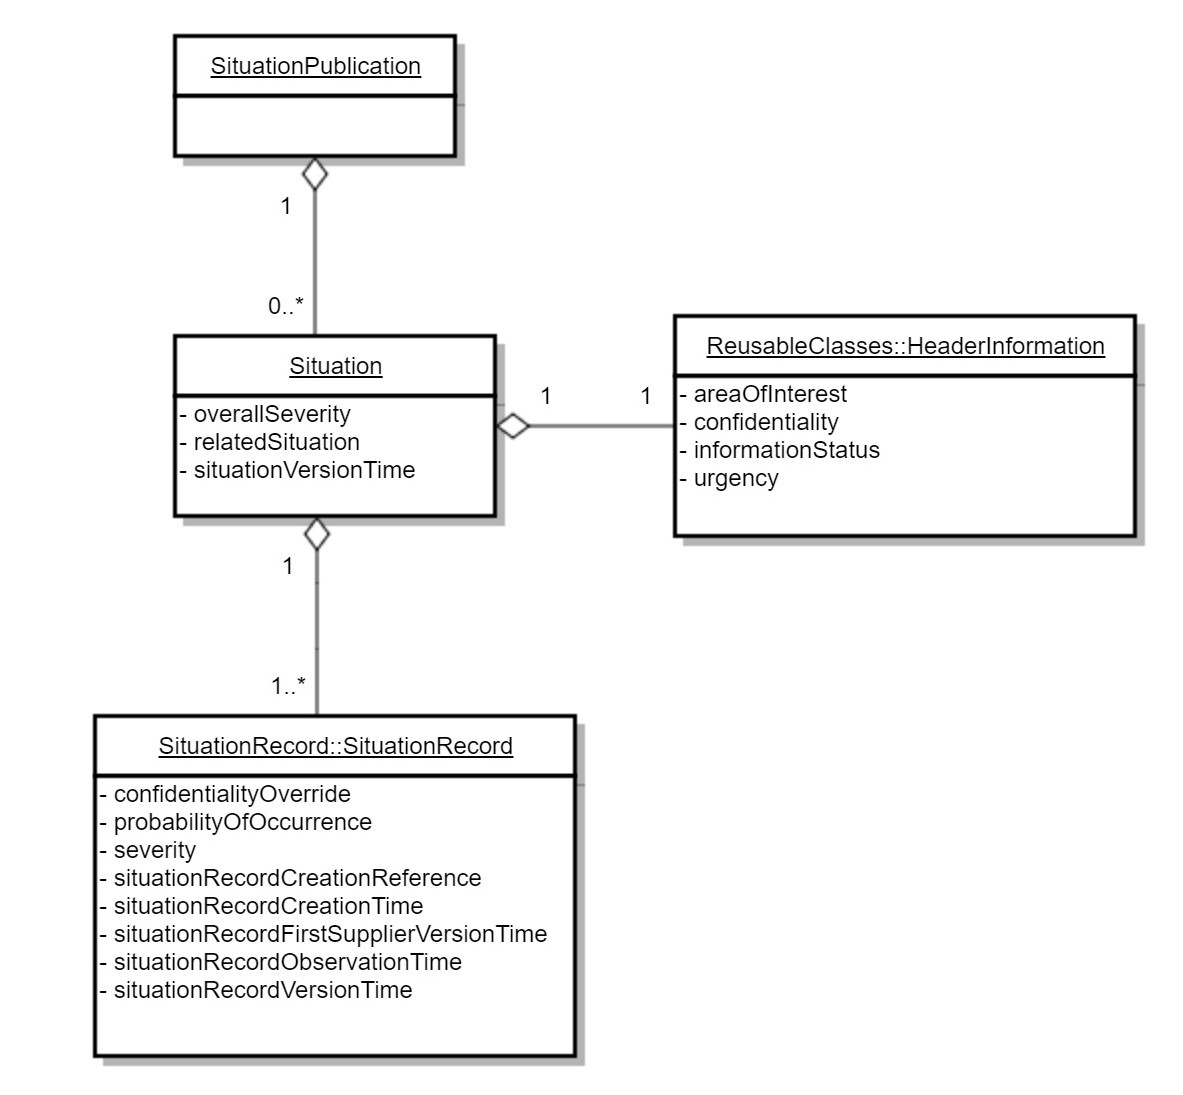
\includegraphics[width=0.7\columnwidth]{images/uml_3_11}
	\end{center}
	\caption{Situation Publication Structure}
	\label{fig:app_uml_3_11}
\end{figure}
\begin{figure}
	\begin{center}
		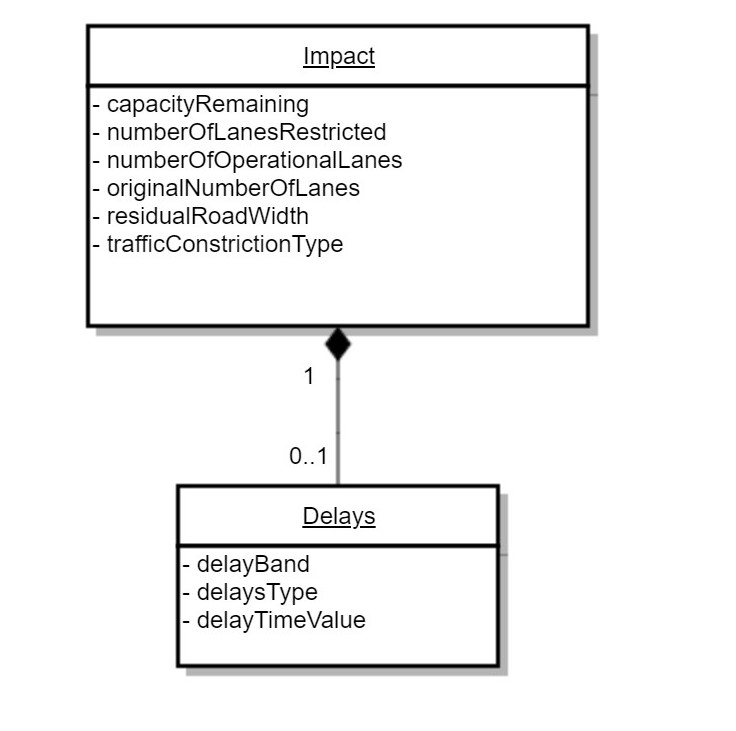
\includegraphics[width=0.45\columnwidth]{images/uml_4_32}
	\end{center}
	\caption{Impact Implementation}
	\label{fig:app_uml_4_32}
\end{figure}
\begin{figure}
	\begin{center}
		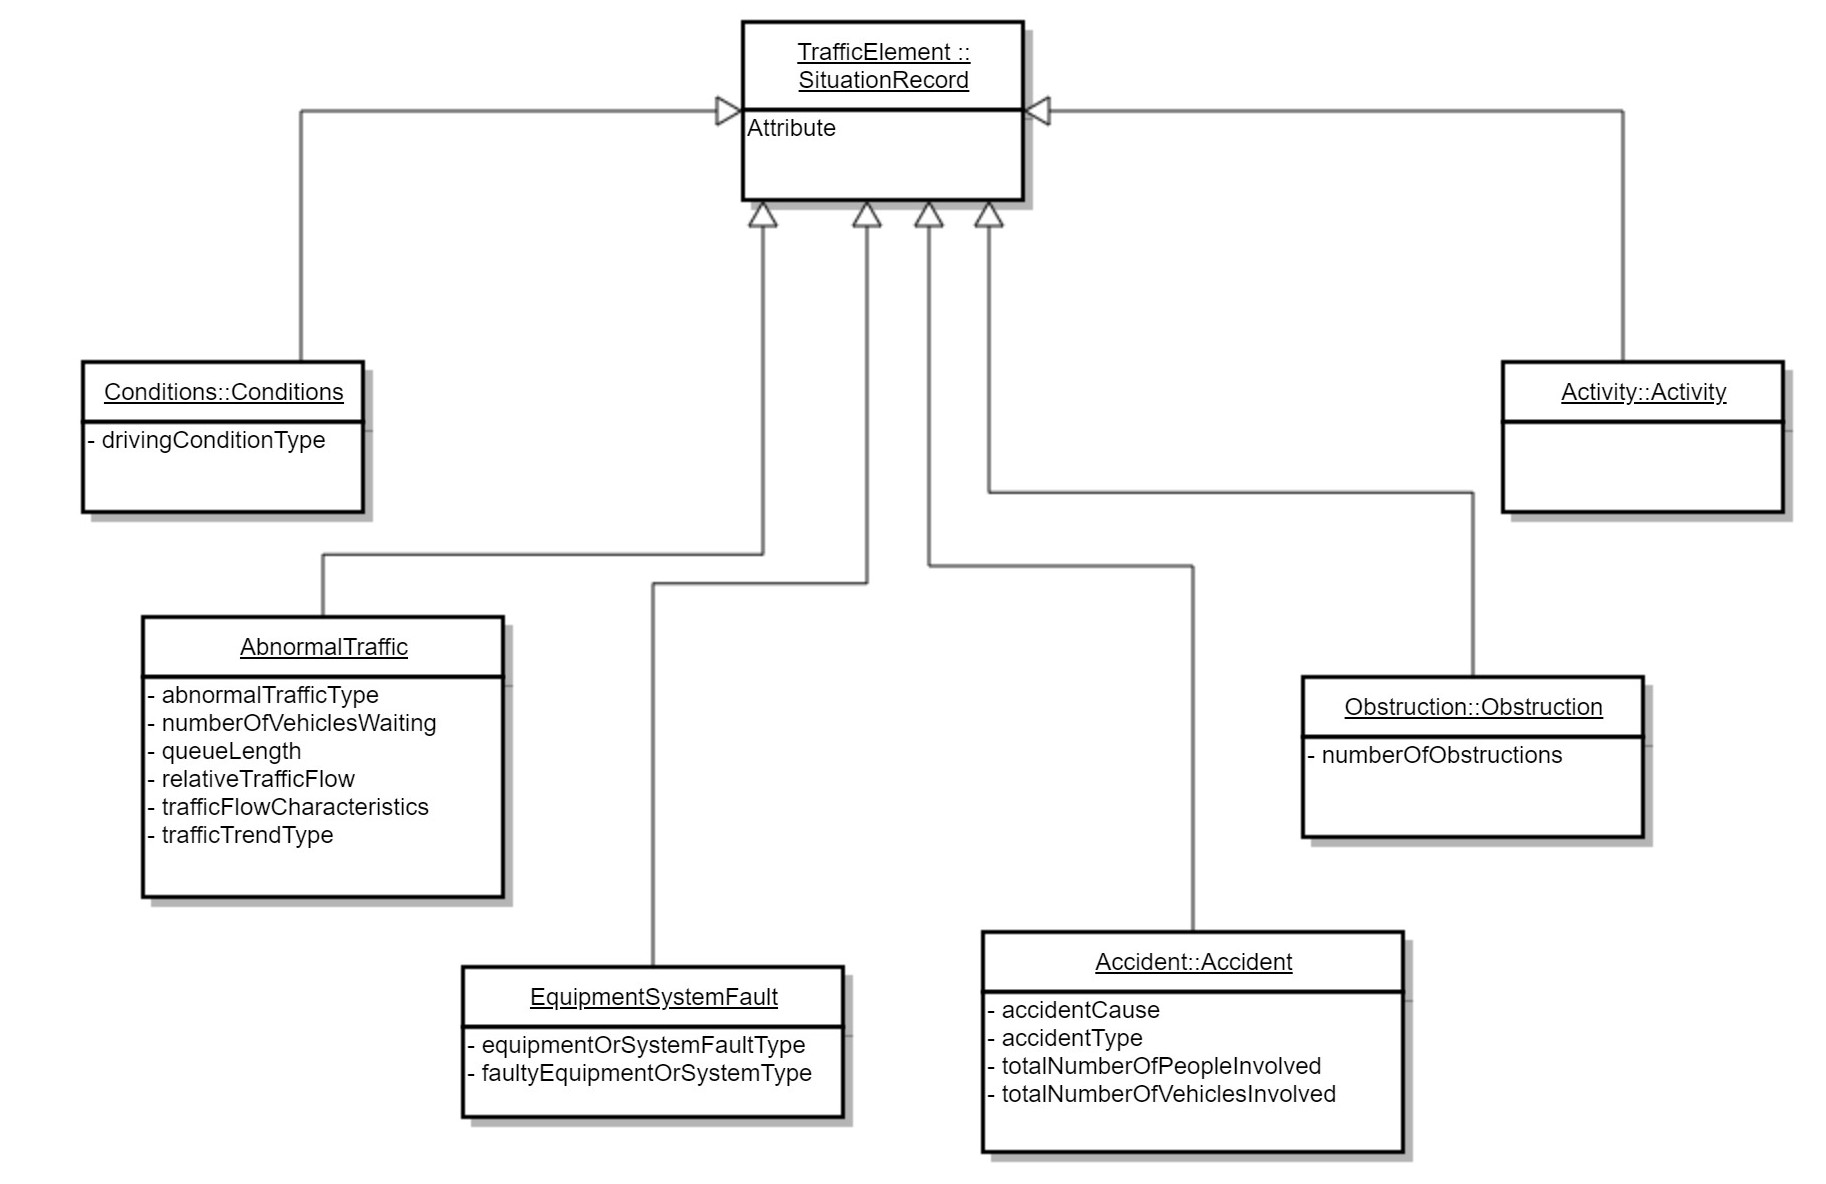
\includegraphics[width=0.85\columnwidth]{images/uml_4_36}
	\end{center}
	\caption{Traffic Element Implementation}
	\label{fig:app_uml_4_36}
\end{figure}
\begin{figure}
	\begin{center}
		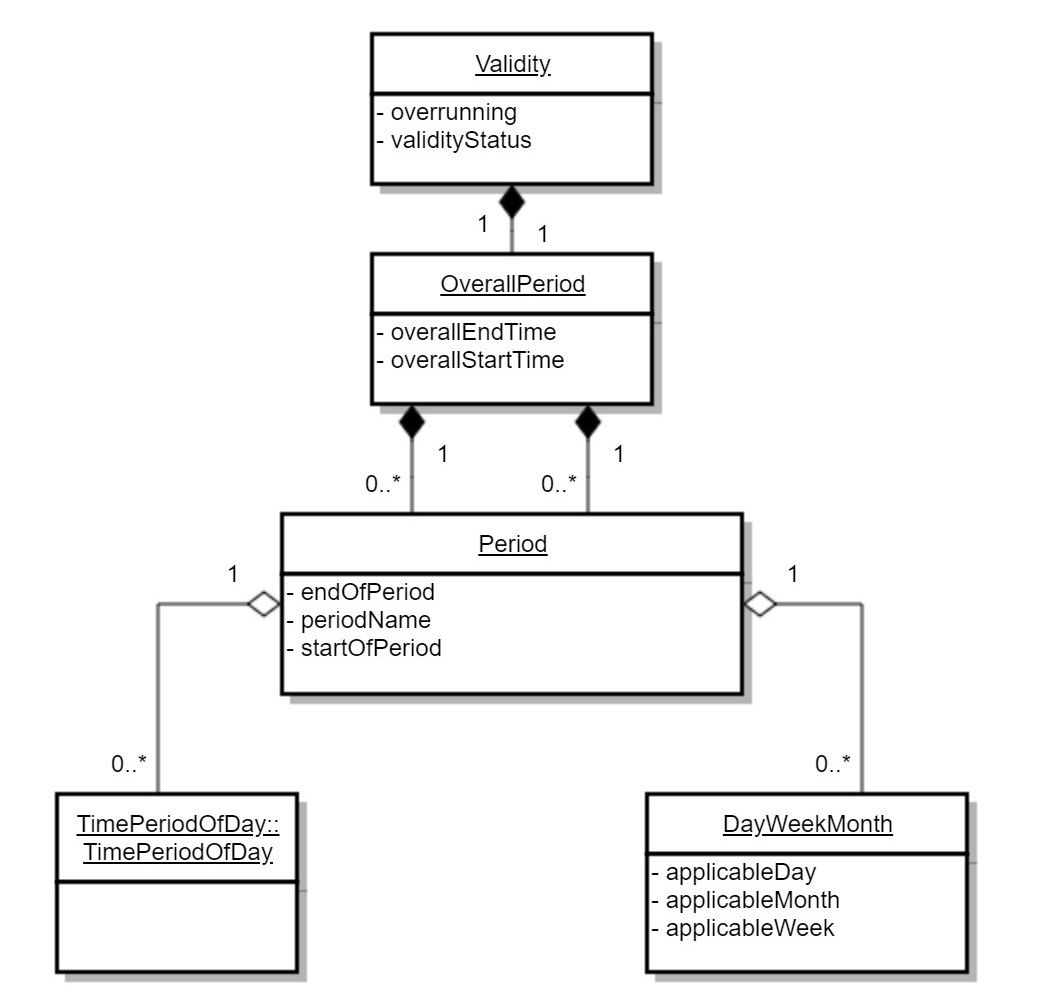
\includegraphics[width=0.6\columnwidth]{images/uml_4_37}
	\end{center}
	\caption{Validity Implementation}
	\label{fig:app_uml_4_37}
\end{figure}
\subsubsection{Standard Extension}
\begin{figure}
	\begin{center}
		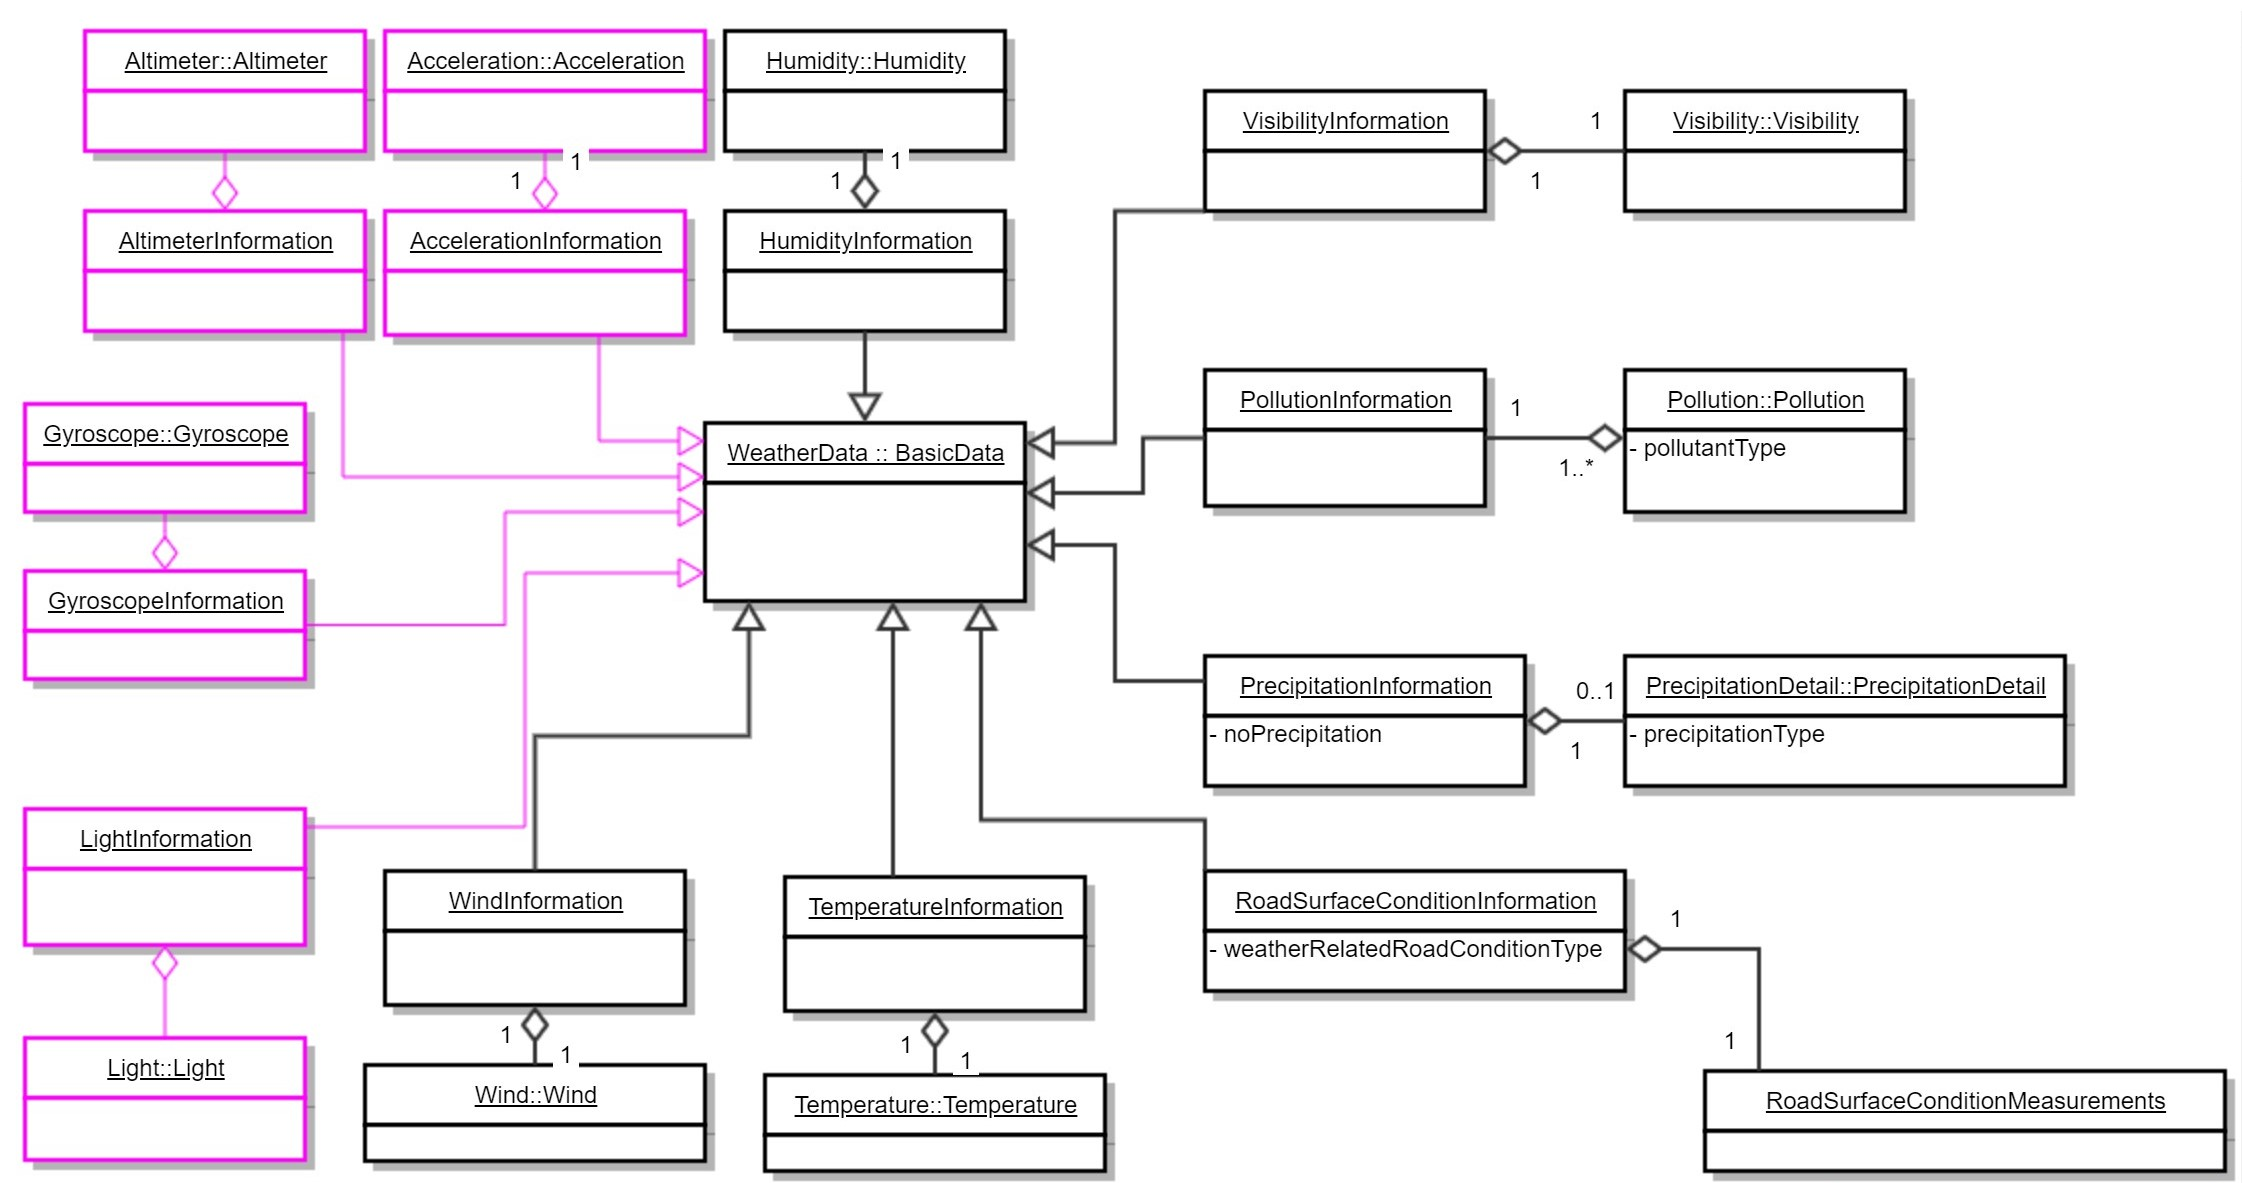
\includegraphics[width=1\columnwidth]{images/uml_4_28_extended}
	\end{center}
	\caption{Level B extension to the DATEX II Standard}
	\label{fig:app_uml_4_28_extended}
\end{figure}

